\section{Customer guide} \label{_cliente}
\subsection{Purpose of the section}
The goal of this section of the document is to describe how a customer should use the interface that EmporioLambda provides.

\subsection{Landing to the web-application}
The only current way to access the application is by direct link: \url{https://d28yg0rufs9lo7.cloudfront.net/}
After accessing the the application by link you will land in the homepage.

\subsection{Layouts}
The application has cross page layouts. The main layout is available in the Hompage, Product List Page, Product Details Page.

\subsubsection{Main Layout} \label{_mainLayout}
The main layout has two navigation bars:

\begin{itemize} 
    \item \textbf{Main NavBar:} this navigation bar contains: 
    \begin{itemize}
        \item \textbf{Company Logo:} when pressed it always redirects to the homepage;
        \item \textbf{Searchbar:} allows to search a specific item in the store;
        \item \textbf{Login button:} when pressed it redirects to the login page;
        \item \textbf{Cart:} when pressed it redirects to the cart page;
    \end{itemize}
    \item \textbf{Categories NavBar:} contains all the categories that are present in the e-commerce. Each category can be pressed and then the application redirects to the products page showing only the products of the selected category;
\end{itemize}

\begin{figure}[H]
    \centering
    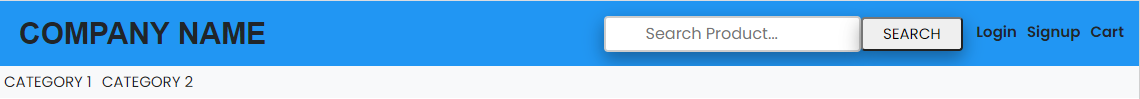
\includegraphics[width=\linewidth]{res/images/cliente/navigationbars.png}
    \caption{Navigation Bars}
\end{figure}

\subsubsection{Alternative Layout}
The alternative layout has only the \textbf{Main NavBar}, refer to \hyperref[_mainLayout]{Main NavBar}. It is used in each other page.

\subsubsection{Footer}
Each page has a footer section where the customer can find useful information about the company.

\begin{figure}[H]
    \centering
    
\includegraphics[width=\linewidth]{res/images/cliente/footer.png}
    \caption{Footer}
\end{figure}

\subsection{Homepage}
This is the first page the customer will see. It contains the highlighted products. Each product has the main image, name and price. When pressed it redirects to the detail page of the specific product.

\begin{figure}[H]
    \centering
    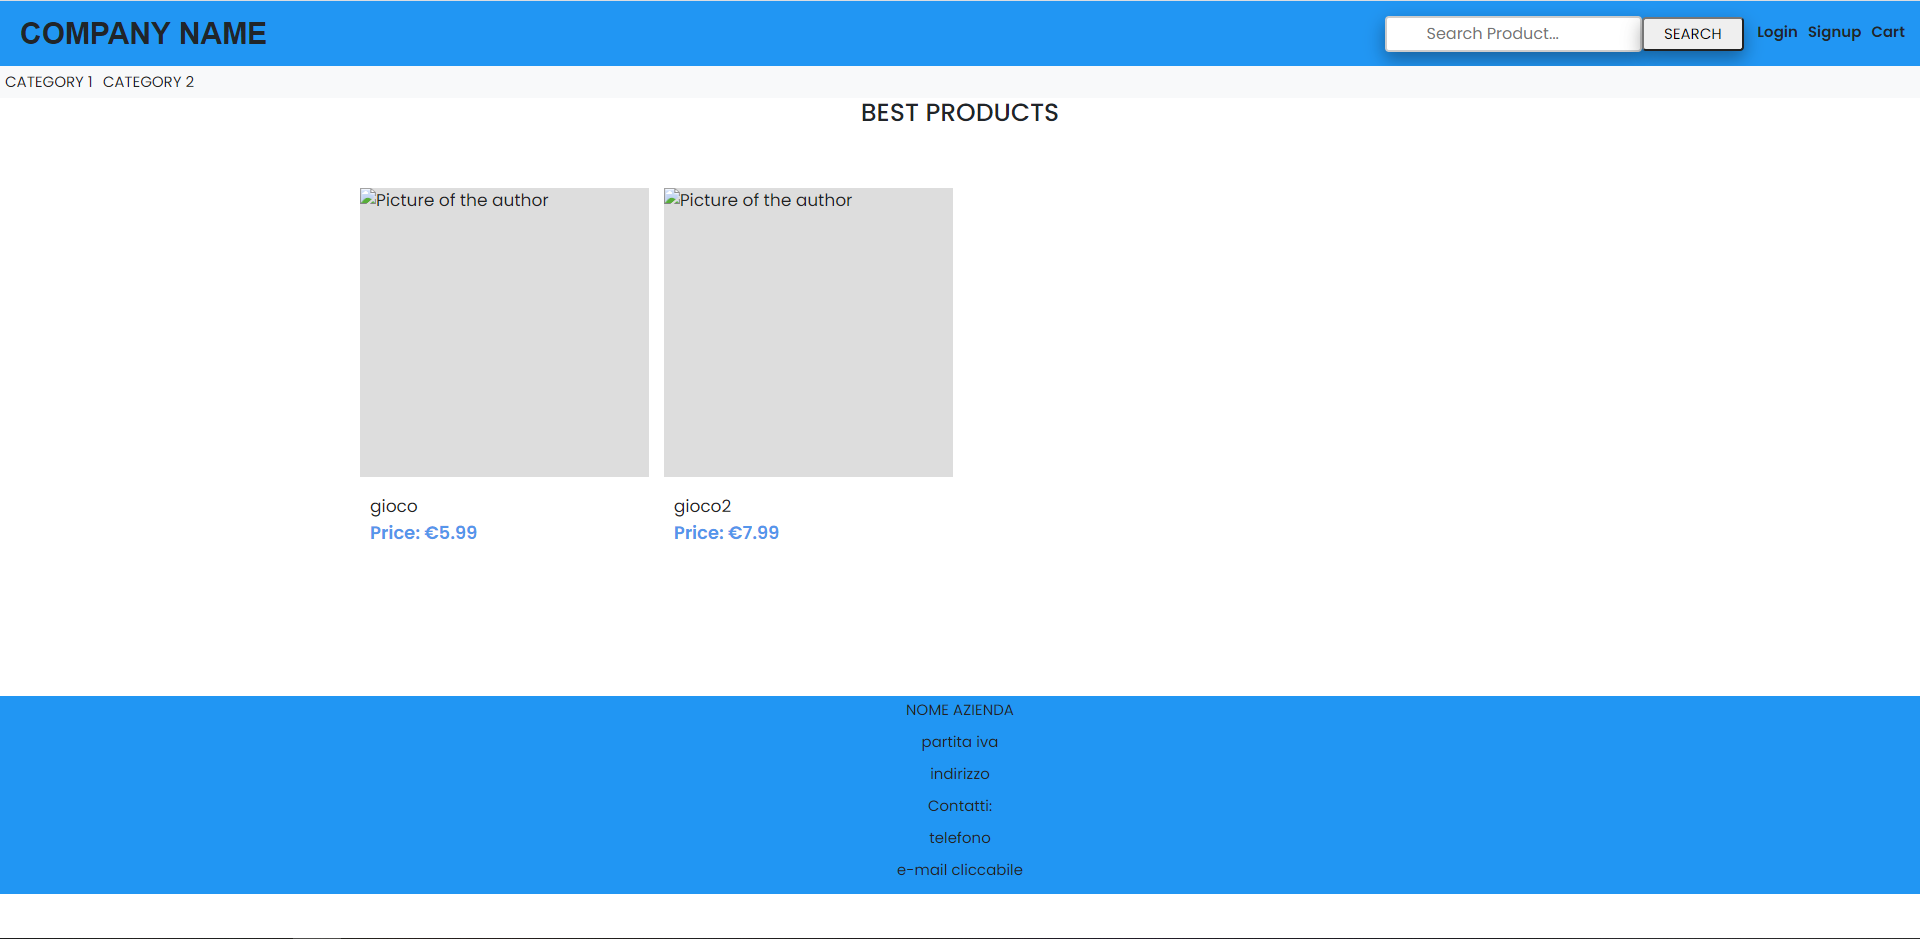
\includegraphics[width=\linewidth]{res/images/cliente/homepage.png}
    \caption{Homepage}
\end{figure}

\subsection{Products Listing Page}
In this page you can find all the products that match with the desired filters applied. To reach this page you have to select a category or just simply search a product by name in the Searchbar.

\begin{figure}[H]
    \centering
    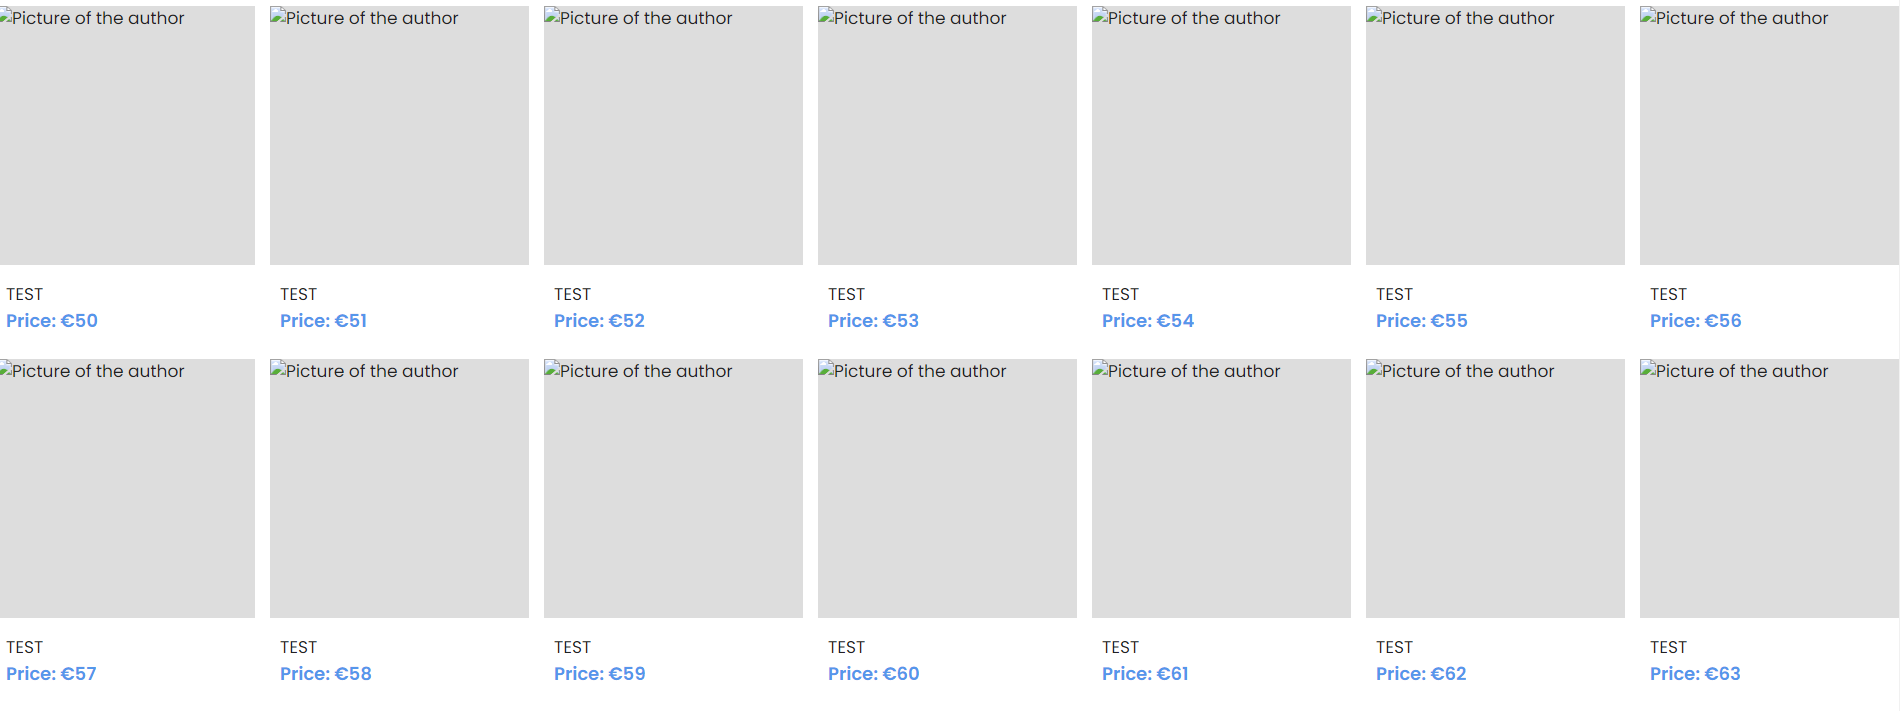
\includegraphics[width=\linewidth]{res/images/cliente/plp.png}
    \caption{Products Listing Page}
\end{figure}

There are also two more filters that can be applied to the list of products.

\begin{itemize} 
    \item \textbf{Filter by cost:} you can set a minimum cost or a maximum cost or both to get a more specific list of products;
    \item \textbf{Order by cost:} you can order the listed products by price. The order can be:
    \begin{itemize}
        \item \textbf{Low to High:} orders the products from the cheapest to the more expensive;
        \item \textbf{High to Low:} orders the products from the more expensive to the cheapest;
    \end{itemize}
\end{itemize}

\subsection{Product Details Page}
In this page you can find all the infos about the selected product.

\begin{figure}[H]
    \centering
    
\includegraphics[width=\linewidth]{res/images/cliente/pdp.png}
    \caption{Product Details Page}
\end{figure}

Main details are:

\begin{itemize} 
    \item \textbf{Product Name}
    \item \textbf{Images}
    \item \textbf{Price} 
    \item \textbf{Description} 
\end{itemize}

Here you can add/remove the product in/from your cart. You can increase the amount of products to add to the cart by pressing the plus (+) button. Same of decreasing the amount by pressing minus (-).

\subsection{Cart}
In this page you can find the cart with all products you added.

\begin{figure}[H]
    \centering
    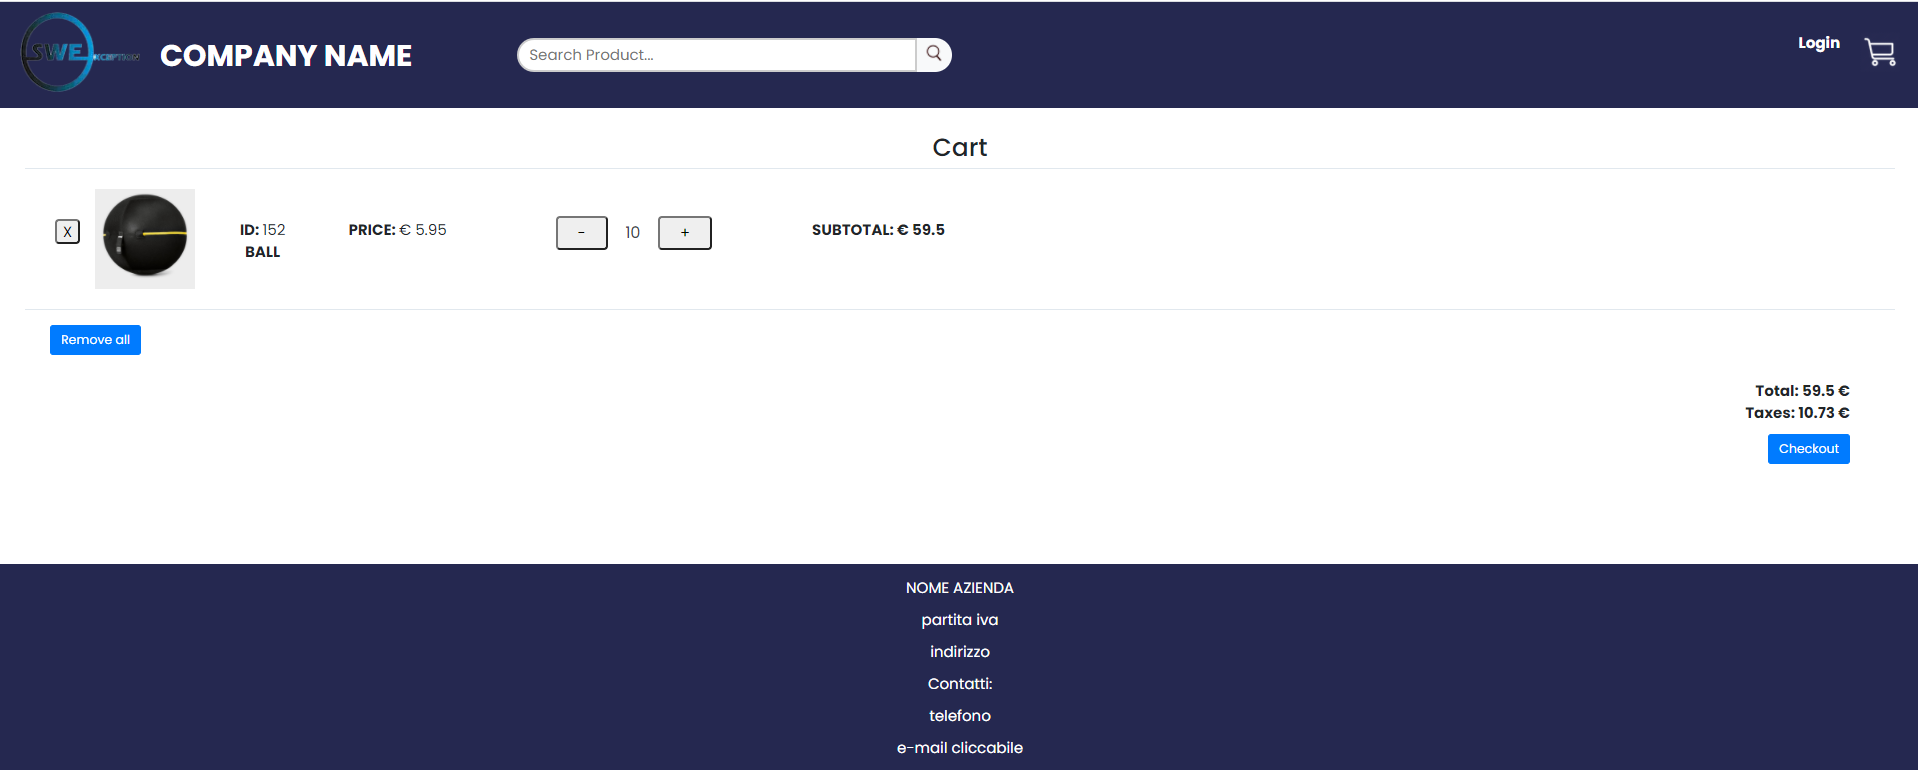
\includegraphics[width=\linewidth]{res/images/cliente/cart.png}
    \caption{Cart}
\end{figure}